\section{Simulation results}\label{sec:results}

\subsection{Detection at a matched false-alarm rate}\label{sec:res-main}

\Cref{tab:detection} and \cref{fig:summary} give the headline comparison. At a per-window false-alarm rate of $10^{-3}$, \qtrace{} raised an alarm on \DetKnownQT\,\% of links under the known attack families, \DetZeroDayQT\,\% under the zero-day families and \DetCompQT\,\% under composite attacks. The strongest comparison method in each group reached \DetKnownBest\,\% (\DetKnownBestName), \DetZeroDayBest\,\% (\DetZeroDayBestName) and \DetCompBest\,\% (\DetCompBestName). The zero-day figure of the quantum-kernel detector should not be read as detection: the same method alarms on \FAHonestQKoneclassSVM\,\% of attack-free links, more often than it alarms on zero-day attacks. The supervised classifier, which was trained on exactly the known families, is the closest competitor on known attacks and falls to \DetZeroDayXGBoostsup\,\% on zero-day families, which is the behaviour one expects from a model that has learned what particular attacks look like rather than what honest links look like. The decoy-state CUSUM, which encodes the consistency check most deployed systems perform, detects only \DetKnownDecoyCUSUM\,\% of known attacks: the decoy-state estimates are noisy functionals of the gains, and stealthy blinding and weak PNS move them by less than their window-to-window fluctuation. The window-level AUROC (\cref{tab:auroc}) gives a similar picture, with \qtrace{} at \AucKnownQT, \AucZeroDayQT{} and \AucCompQT{} for the three groups, with one exception: on long links the supervised classifier reaches \AucShiftXGB{} against \AucShiftQT{} for \qtrace{}. AUROC weights all thresholds equally, whereas operation happens at a low false-alarm rate, where the detection rates of \cref{tab:detection} are the relevant measure.

\begin{table}[!tbp]
\centering
\caption{Percentage of attacked links detected, by attack group, and percentage of attack-free test links with at least one alarm (FA), at a per-window false-alarm rate of $10^{-3}$ set on validation links. ``Long links'' is the 60 to 120\,km regime absent from training. Mean\,$\pm$\,95\,\% confidence interval over \NSeeds{} held-out seeds.}
\label{tab:detection}
\small
\resizebox{\textwidth}{!}{\begin{tabular}{lccccccc}
\toprule
Method & Known & Zero-day & Composite & Long links & FA honest & FA loss & FA long \\
\midrule
\textbf{Q-TRACE} & \textbf{63.6\,$\pm$\,6.6} & \textbf{28.0\,$\pm$\,2.5} & \textbf{65.3\,$\pm$\,9.1} & \textbf{32.0\,$\pm$\,7.5} & \textbf{5.2\,$\pm$\,3.8} & \textbf{0.0\,$\pm$\,0.0} & \textbf{3.2\,$\pm$\,2.2} \\
XGBoost (sup.) & 51.2\,$\pm$\,8.5 & 0.6\,$\pm$\,0.6 & 42.3\,$\pm$\,10.8 & 24.4\,$\pm$\,9.2 & 0.8\,$\pm$\,1.4 & 8.8\,$\pm$\,6.5 & 0.0\,$\pm$\,0.0 \\
QBER CUSUM & 27.2\,$\pm$\,5.3 & 1.3\,$\pm$\,2.5 & 21.0\,$\pm$\,3.8 & 9.8\,$\pm$\,3.7 & 1.2\,$\pm$\,2.2 & 1.6\,$\pm$\,2.7 & 0.0\,$\pm$\,0.0 \\
Decoy CUSUM & 2.5\,$\pm$\,2.8 & 0.0\,$\pm$\,0.0 & 0.3\,$\pm$\,0.9 & 0.0\,$\pm$\,0.0 & 0.0\,$\pm$\,0.0 & 3.2\,$\pm$\,2.2 & 0.0\,$\pm$\,0.0 \\
QBER static & 13.1\,$\pm$\,6.0 & 1.7\,$\pm$\,1.3 & 11.7\,$\pm$\,7.3 & 50.7\,$\pm$\,7.4 & 2.8\,$\pm$\,2.8 & 0.8\,$\pm$\,2.2 & 45.6\,$\pm$\,16.7 \\
Autoencoder & 3.0\,$\pm$\,2.7 & 0.0\,$\pm$\,0.0 & 1.3\,$\pm$\,1.7 & 0.9\,$\pm$\,1.5 & 0.0\,$\pm$\,0.0 & 4.0\,$\pm$\,8.6 & 0.0\,$\pm$\,0.0 \\
Isolation forest & 3.6\,$\pm$\,4.6 & 0.4\,$\pm$\,1.1 & 5.0\,$\pm$\,8.5 & 0.0\,$\pm$\,0.0 & 0.0\,$\pm$\,0.0 & 12.0\,$\pm$\,8.6 & 0.0\,$\pm$\,0.0 \\
One-class SVM & 0.0\,$\pm$\,0.0 & 0.0\,$\pm$\,0.0 & 0.0\,$\pm$\,0.0 & 0.0\,$\pm$\,0.0 & 0.0\,$\pm$\,0.0 & 0.0\,$\pm$\,0.0 & 0.0\,$\pm$\,0.0 \\
QK one-class SVM & 5.7\,$\pm$\,2.5 & 6.7\,$\pm$\,2.4 & 4.3\,$\pm$\,2.8 & 8.9\,$\pm$\,6.2 & 10.4\,$\pm$\,3.2 & 12.8\,$\pm$\,4.2 & 7.2\,$\pm$\,5.4 \\
\bottomrule
\end{tabular}
}
\end{table}

\begin{figure}[!tbp]
\centering
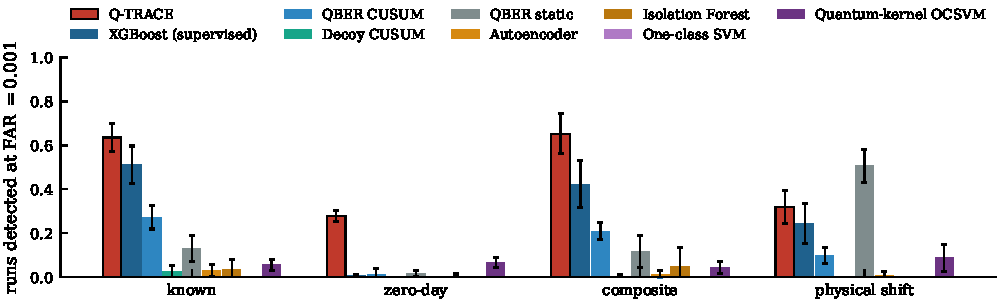
\includegraphics[width=\textwidth]{figures/fig5_detection_summary.pdf}
\caption{Fraction of attacked links detected at a per-window false-alarm rate of $10^{-3}$, by attack group. Error bars are 95\,\% confidence intervals over held-out seeds.}
\label{fig:summary}
\end{figure}

\Cref{fig:traces} shows what these numbers mean on individual links. For a PNS attack that leaves the gain and QBER unchanged, the \qtrace{} statistic crosses its threshold within a few windows of onset, while the QBER and decoy-state CUSUMs, scaled to their own thresholds, stay below one. For stealthy blinding, which reproduces gain and QBER by construction, the alarm is driven by the vanishing double clicks and vacuum clicks. For the modulated RNG attack the energy and setting channels respond, whereas monitors built on time-averaged balance do not.

\begin{figure}[!tbp]
\centering
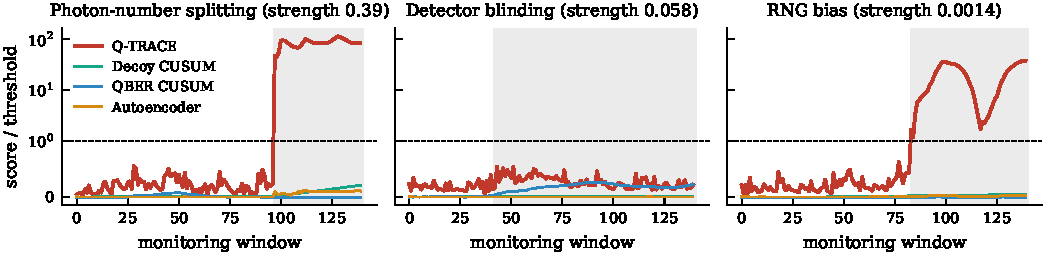
\includegraphics[width=\textwidth]{figures/fig2_example_traces.pdf}
\caption{Alarm statistics divided by their thresholds on three test links (shaded: attack active). Values above one are alarms. The vertical axis is linear below one and logarithmic above.}
\label{fig:traces}
\end{figure}

\subsection{Attack families and strength}\label{sec:res-family}

\Cref{fig:strength} resolves detection by family and attack strength, and \cref{tab:perfamily} lists the per-family detection rates of all methods. Intercept--resend is the one family for which a QBER monitor is close to optimal, because the attack does nothing except raise the QBER; the QBER CUSUM detects \FamInterceptresendQC\,\% and \qtrace{} \FamInterceptresendQT\,\%. For PNS (\FamPNSQT\,\% against \FamPNSXGB\,\% for the supervised classifier and \FamPNSQC\,\% for the QBER CUSUM) and blinding (\FamBlindingQT\,\% against \FamBlindingXGB\,\%) the advantage comes from constraints that the QBER does not see. Among the zero-day families, \qtrace{} detects \FamRNGbiasQT\,\% of RNG-bias attacks, for which every comparison method stays near its false-alarm level, and \FamTimeshiftQT\,\% of time-shift attacks. Detection of Trojan-horse probes with back-scatter is low for every method (\qtrace{} \FamTrojanhorseQT\,\%): the back-scattered background is small compared with the afterpulse background of most links, and the theory below shows that the information available is correspondingly small.

\begin{figure}[!tbp]
\centering
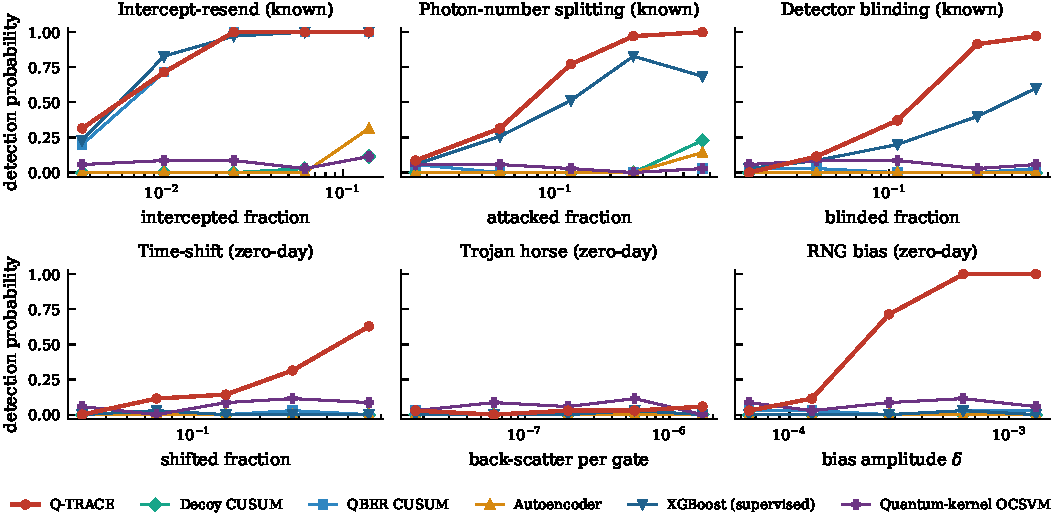
\includegraphics[width=\textwidth]{figures/fig3_detection_vs_strength.pdf}
\caption{Detection probability at a per-window false-alarm rate of $10^{-3}$ against attack strength, in quintile bins of strength. Pooled over held-out seeds.}
\label{fig:strength}
\end{figure}

\begin{table}[!htb]
\centering
\caption{Percentage of attacked test links detected, per attack family, at a per-window false-alarm rate of $10^{-3}$ (mean over seeds; best method per row in bold).}
\label{tab:perfamily}
\small
\begin{tabular}{lccccccccc}
\toprule
Family & \rotatebox{70}{Q-TRACE} & \rotatebox{70}{XGBoost (sup.)} & \rotatebox{70}{QBER CUSUM} & \rotatebox{70}{Decoy CUSUM} & \rotatebox{70}{QBER static} & \rotatebox{70}{Autoencoder} & \rotatebox{70}{Isolation forest} & \rotatebox{70}{One-class SVM} & \rotatebox{70}{QK one-class SVM} \\
\midrule
Intercept-resend & \textbf{80.6} & 80.6 & 78.3 & 2.9 & 36.6 & 6.3 & 9.1 & 0.0 & 7.4 \\
PNS & \textbf{62.9} & 46.9 & 1.7 & 4.6 & 1.7 & 2.9 & 1.7 & 0.0 & 3.4 \\
Blinding & \textbf{47.4} & 26.3 & 1.7 & 0.0 & 1.1 & 0.0 & 0.0 & 0.0 & 6.3 \\
Time-shift & \textbf{24.0} & 0.6 & 0.6 & 0.0 & 2.9 & 0.0 & 0.6 & 0.0 & 6.9 \\
Trojan horse & 2.9 & 0.6 & 1.1 & 0.0 & 1.1 & 0.0 & 0.6 & 0.0 & \textbf{5.7} \\
RNG bias & \textbf{57.1} & 0.6 & 2.3 & 0.0 & 1.1 & 0.0 & 0.0 & 0.0 & 7.4 \\
PNS + blinding & \textbf{81.0} & 57.0 & 1.0 & 1.0 & 2.0 & 2.0 & 6.0 & 0.0 & 3.0 \\
Time-shift + Trojan & \textbf{29.0} & 3.0 & 0.0 & 0.0 & 1.0 & 0.0 & 0.0 & 0.0 & 6.0 \\
IR + RNG bias & \textbf{86.0} & 67.0 & 62.0 & 0.0 & 32.0 & 2.0 & 9.0 & 0.0 & 4.0 \\
\bottomrule
\end{tabular}

\end{table}

\subsection{Delay against the information-theoretic bound}\label{sec:res-bound}

\Cref{fig:bound} places every detected attack on the plane of its own delay bound $\log(1/\alpha)/(N\Dstar)$ and its observed delay. The median delay of \qtrace{} lies on the bound for attacks with bounds below one window and stays within a small factor of it up to bounds of about ten windows. The QBER CUSUM and the supervised classifier detect fewer attacks, and those they detect require between one and two orders of magnitude more data than the bound. \Cref{tab:bound} quantifies the same effect as detection rates: for attacks whose bound is below one window, \qtrace{} detects \BoundLtOneQT\,\% (the supervised classifier \BoundLtOneXGB\,\%, the QBER CUSUM \BoundLtOneQC\,\%); for bounds between one and ten windows the rates are \BoundOneTenQT\,\%, \BoundOneTenXGB\,\% and \BoundOneTenQC\,\%.

\begin{figure}[!htb]
\centering
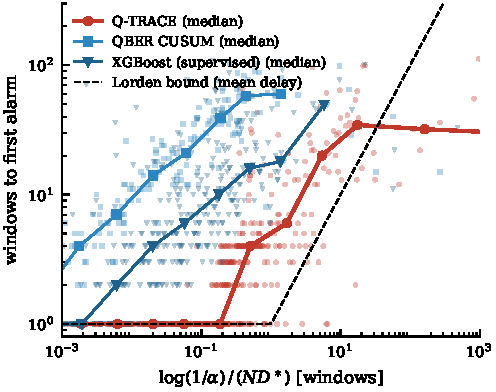
\includegraphics[width=0.56\textwidth]{figures/fig4_delay_vs_lorden_bound.pdf}
\caption{Windows of post-onset data needed for the first alarm against the information-theoretic bound of \cref{prop:lorden} for each detected attack (points) and binned medians (lines). The dashed line is $\max(1,\text{bound})$. The bound constrains the mean delay, so individual runs can fall below it.}
\label{fig:bound}
\end{figure}

\begin{table}[!tbp]
\centering
\caption{Percentage of attacked links detected, grouped by the delay bound $\log(1/\alpha)/(N\Dstar)$ of each run in windows, at $\alpha=10^{-3}$. Runs are pooled over seeds; the last row gives the number of attack runs per bin.}
\label{tab:bound}
\small
\begin{tabular}{lcccc}
\toprule
Method & bound $<1$ & bound 1--10 & bound 10--100 & bound $>100$ \\
\midrule
\textbf{Q-TRACE} & \textbf{93.7} & \textbf{25.4} & \textbf{7.8} & \textbf{2.6} \\
XGBoost (sup.) & 62.0 & 6.4 & 1.8 & 0.3 \\
QBER CUSUM & 31.7 & 3.4 & 1.8 & 1.0 \\
Decoy CUSUM & 2.6 & 0.0 & 0.0 & 0.0 \\
QBER static & 19.9 & 13.6 & 11.5 & 10.9 \\
Autoencoder & 3.7 & 0.0 & 0.0 & 0.0 \\
Isolation forest & 4.1 & 0.0 & 0.0 & 0.3 \\
One-class SVM & 0.0 & 0.0 & 0.0 & 0.0 \\
QK one-class SVM & 6.7 & 6.1 & 4.6 & 8.6 \\
\midrule
Attack runs & 492 & 264 & 217 & 302 \\
\bottomrule
\end{tabular}

\end{table}

The gap between \qtrace{} and the bound for bounds between one and a hundred windows has a clear origin. The bound assumes a stationary honest link, whereas the twin drifts. In a development run on seed 1 with all nuisance drift switched off, the first version of the monitor detected 74\,\% of attacked links and 93\,\% of those with bounds below 20 windows; with drift switched on the same monitor detected 39\,\%, and the moving-reference channels of \cref{sec:moving} raised this to 59\,\% before the configuration was frozen. Slow honest drift, not the statistical efficiency of the monitor, is therefore the binding limit in the realistic regime. An extension of the bound to drifting pre-change laws is left for future work.

\subsection{False alarms, benign faults and unseen regimes}\label{sec:res-fa}

\Cref{fig:fa} and the last three columns of \cref{tab:detection} show how often each method alarms on attack-free links. Over the 140 monitoring windows of a link the per-window rate of $10^{-3}$ corresponds to a run-level rate of roughly 13\,\% for independent windows; on nominal honest links all methods stay below this, \qtrace{} at \FAHonestQT\,\%. \qtrace{} raised an alarm on \FALossQT\,\% of links with benign loss faults, because a loss step changes only the nuisance parameter; the isolation forest (\FALossIsolationforest\,\%), the quantum-kernel one-class SVM (\FALossQKoneclassSVM\,\%) and the autoencoder (\FALossAutoencoder\,\%) treat the same steps as anomalies. On honest long links, the static QBER threshold alarms on \FALongQBERstatic\,\% of runs because the honest QBER of long links can exceed 11\,\%; its apparently high detection rate in the long-link regime (\DetShiftQBERstatic\,\%) is an artefact of this and not evidence of detection. \qtrace{} alarms on \FALongQT\,\% of honest long links and detects \DetShiftQT\,\% of attacks there, lower than in the nominal regime because fewer clicks per window carry less information. Dark-count faults are detected by none of the methods with high probability: with afterpulse backgrounds of order $10^{-4}$ per gate, a rise of the intrinsic dark-count probability from $10^{-6}$ by a factor of a few changes the total background only marginally.

\begin{figure}[!tbp]
\centering
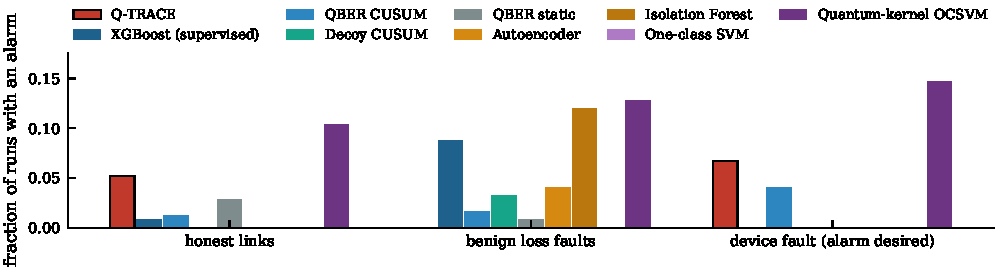
\includegraphics[width=\textwidth]{figures/fig6_false_alarms.pdf}
\caption{Fraction of test links with at least one alarm at a per-window false-alarm rate of $10^{-3}$: attack-free links, links with benign loss faults (steps or ramps of 0.5 to 3\,dB) and links with a dark-count fault, where an alarm is desirable.}
\label{fig:fa}
\end{figure}

\subsection{Physical attribution of alarms}\label{sec:res-attr}

Because the score channel is built from physical directions, an alarm comes with a statement of which constraint was violated. \Cref{fig:attr} shows, for each attack family, the device parameter with the largest standardised displacement at the first alarm. Blinding and PNS alarms are most often attributed to the double-click direction (\AttrBlindingShare\,\% and \AttrPNSShare\,\% respectively), consistent with blinded detectors that never double-click and with the altered multi-photon statistics of a lossless PNS channel. Intercept--resend alarms are most often attributed to an optical-error direction (\AttrInterceptresendShare\,\%), as \cref{eq:ir} predicts. The attribution is a diagnostic aid, not a classifier: it was not tuned on attack data, and it does not apply to the RNG attack, whose alarms come from the setting channel.

\begin{figure}[!htb]
\centering
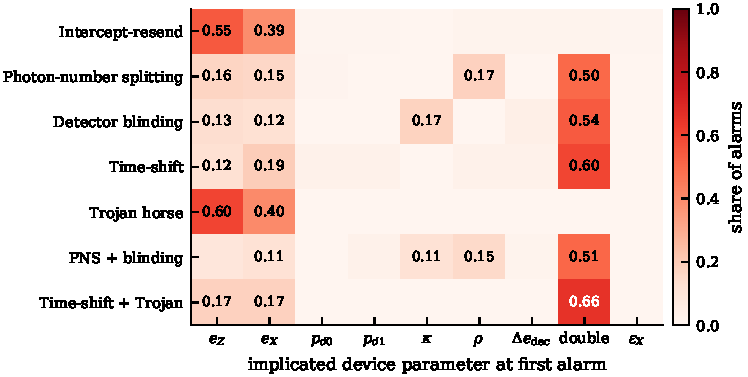
\includegraphics[width=0.78\textwidth]{figures/fig7_physical_attribution.pdf}
\caption{Device parameter implicated at the first alarm of \qtrace{}, by attack family (share of detected runs; entries below 0.1 not printed). RNG bias is excluded because attribution is defined over device directions only.}
\label{fig:attr}
\end{figure}

\subsection{The quantum-kernel baseline}\label{sec:res-qk}

The one-class SVM on a quantum fidelity kernel performs close to chance (AUROC \AucKnownQK{} on known attacks) and has the highest false-alarm rate on loss faults. We do not read this as a statement about quantum machine learning in general. The kernel acts on a six-dimensional projection of standardised telemetry scalars, and \cref{prop:lorden} implies that no representation of those scalars, quantum or classical, can extract information that the scalars do not contain; much of the relevant information sits in cells, such as vacuum double clicks, that the scalars summarise poorly. The result does suggest that, for this problem, the choice of statistic matters more than the choice of model class.
